\documentclass[11pt]{article}
\usepackage[a4paper,margin=25mm,headheight=14pt]{geometry}
\usepackage[T1]{fontenc}
\usepackage{lmodern,microtype}
\usepackage{amsmath,amssymb,amsthm,mathtools}
\usepackage{graphicx,booktabs,array,longtable,enumitem}
\usepackage[dvipsnames]{xcolor}
\usepackage{hyperref,fancyhdr,listings}
\definecolor{navy}{HTML}{18334D}
\definecolor{teal}{HTML}{007F86}
\hypersetup{colorlinks=true,linkcolor=navy,urlcolor=teal,citecolor=teal,
 pdftitle={Farthest points and intrinsic diameter of a cuboid},
 pdfauthor={Prepared for Vladimir Reshetnikov}}
\pagestyle{fancy}
\fancyhf{}
\fancyhead[L]{\small Farthest points on a cuboid}
\fancyhead[R]{\small Intrinsic surface distance}
\fancyfoot[C]{\thepage}
\setlength{\parskip}{4pt}
\setlength{\parindent}{0pt}
\setlength{\emergencystretch}{2em}
\setlist{itemsep=3pt,topsep=4pt}
\newtheorem{theorem}{Theorem}[section]
\newtheorem{lemma}[theorem]{Lemma}
\newtheorem{proposition}[theorem]{Proposition}
\newtheorem{corollary}[theorem]{Corollary}
\theoremstyle{definition}
\newtheorem{definition}[theorem]{Definition}
\newtheorem{remark}[theorem]{Remark}
\newcommand{\R}{\mathbb R}
\newcommand{\surf}{\Sigma}
\newcommand{\spq}[1]{\sqrt{\max\{0,#1\}}}
\newcommand{\dist}{d_{\surf}}
\newcommand{\sqzero}{Q_0}
\newcommand{\sqone}{Q_1}
\newcommand{\vertexecc}{E}
\newcommand{\diameter}{D}
\lstset{basicstyle=\small\ttfamily,breaklines=true,columns=fullflexible,
 frame=single,rulecolor=\color{black!15},backgroundcolor=\color{black!2},
 showstringspaces=false}
\title{\color{navy}\bfseries Farthest points and intrinsic diameter\\[3pt]
of a rectangular cuboid}
\author{A complete geometric argument and a Lean formalization plan\\[4pt]
\small Prepared for Vladimir Reshetnikov}
\date{19 November 2026}
\begin{document}
\maketitle
\begin{abstract}
The farthest surface point from a vertex of a cuboid need not be the
opposite vertex. We give its coordinates and distance in two elementary
cases. When both endpoints are free, a maximizing pair is centrally
opposite and lies on the two faces perpendicular to a longest edge.
Its distance and coordinates follow from one strictly increasing scalar
equation, with a simple exact test for when opposite vertices suffice.
We prove the continuous-path reductions, enumerate the relevant
unfoldings, check that invalid unfoldings cannot undercut the answer,
and solve both optimizations. The unrestricted formula agrees with the
published result of Nikonorov and Nikonorova.

The archive also contains a high-precision calculator, an independent
enumeration of valid face unfoldings, reproducible checks, figures, and
a Lean 4 scaffold. The Lean scaffold is an explicitly unfinished,
uncompiled formalization outline; the human-readable proofs and the
executed computational checks are separate deliverables.
\end{abstract}
\setcounter{tocdepth}{1}
\tableofcontents
\newpage

\section{Coordinates and the answers}

Throughout, all three side lengths are positive. Relabel the axes so that
\[
0<a\le b\le c,\qquad
B=[0,a]\times[0,b]\times[0,c],\qquad \surf=\partial B.
\]
For the first question, put the selected vertex at \(O=(0,0,0)\), with
the positive coordinate axes pointing along its three incident edges.
If the original side lengths were not sorted, permute the resulting
coordinates back to the original axes. For a selected vertex having a
global coordinate equal to its side length, reflect the corresponding
local coordinate. Thus the sorting is only a choice of notation.

The length of a continuous curve \(\gamma:[0,1]\to\R^3\) is
\[
\operatorname{Len}(\gamma)=
\sup_{0=t_0<\cdots<t_n=1}
\sum_{i=1}^{n}\|\gamma(t_i)-\gamma(t_{i-1})\|_2.
\]
It may be infinite. The surface distance is
\[
\dist(P,Q)=\inf\{\operatorname{Len}(\gamma):
\gamma(0)=P,\ \gamma(1)=Q,\ \gamma([0,1])\subseteq\surf\}.
\]
Every curve in this definition stays on the surface, including at edges.
The straight spatial diagonal through the interior is inadmissible.

Write
\[
\sqzero=(a+b)^2+c^2,\qquad
H=2c^2-2bc-ac-ab,\qquad
\delta=\frac{a(c-b)}{2c},
\]
and define
\[
V=(a,b,c),\qquad W=(a-\delta,b-\delta,c),\qquad
\sqone=\frac{(b^2+c^2)(a^2+2ac+2c^2)}{2c^2}.
\]

\subsection{One endpoint is a prescribed vertex}

\begin{theorem}[Fixed-vertex answer]\label{thm:vertex}
The maximum distance from \(O\) is
\[
\boxed{\ \vertexecc=\max_{Y\in\surf}\dist(O,Y)
      =\sqrt{\max\{\sqzero,\sqone\}}\ }.
\]
A maximizing target and the achieved distance are
\[
\boxed{
\begin{array}{c|c|c}
\text{condition}&Y&\dist(O,Y)\\ \hline
H\le0&(a,b,c)&\sqrt{(a+b)^2+c^2}\\[2pt]
H>0&
\left(a-\dfrac{a(c-b)}{2c},\
b-\dfrac{a(c-b)}{2c},\ c\right)&
\sqrt{\dfrac{(b^2+c^2)(a^2+2ac+2c^2)}{2c^2}}
\end{array}}
\]
For \(H<0\), \(V\) is the unique farthest point. For \(H>0\), \(W\) is
the unique farthest point. At \(H=0\), precisely \(V\) and \(W\) tie.
\end{theorem}

The transition can equivalently be expressed as
\[
c=\frac{2b+a+\sqrt{4b^2+12ab+a^2}}4.
\]
The signs in the two-case formula follow from the factorization
\begin{equation}\label{eq:vertex-factor}
\sqone-\sqzero=\frac{a(c-b)H}{2c^2}.
\end{equation}
If \(c=b\), then \(W=V\) and \(H=-2ab<0\), so the formula includes
equal side lengths without an exception.

\subsection{Both endpoints may vary}

For \(T\ge\sqzero\), define
\begin{equation}\label{eq:F}
F(T)=\spq{T-(a+c)^2}
    +\spq{T-(b+c)^2}
    +\sqrt{2T-(a+b+c)^2}.
\end{equation}
The last radical is real: at the left endpoint its radicand is
\((a+b-c)^2\). The function \(F\) is continuous and strictly increasing.

\begin{theorem}[Unrestricted answer]\label{thm:diam}
Let \(\diameter=\max_{X,Y\in\surf}\dist(X,Y)\).

If \(F(\sqzero)\ge c\), then
\[
\boxed{\ \diameter=\sqrt{\sqzero},\qquad X=(0,0,0),\quad
Y=(a,b,c).\ }
\]

If \(F(\sqzero)<c\), there is a unique
\[
T_*\in\bigl(\sqzero,(a+c)^2+b^2\bigr)
\quad\text{such that}\quad F(T_*)=c.
\]
Put
\begin{equation}\label{eq:witness}
u=\spq{T_*-(b+c)^2},\quad v=\spq{T_*-(a+c)^2},
\quad x=\frac{a-u}{2},\quad y=\frac{b-v}{2}.
\end{equation}
Then
\[
\boxed{\ \diameter=\sqrt{T_*},\qquad
X=(x,y,0),\quad Y=(a-x,b-y,c).\ }
\]
Here \(0<x\le a/2\) and \(0<y<b/2\), so both points lie in the
relative interiors of the indicated faces.
\end{theorem}

An exact monotone equation with a specified unique root is a complete
real-number specification. It also makes numerical evaluation easy:
bisection on the displayed finite interval finds the length and
coordinates. Section~\ref{sec:radicals} gives elementary radical formulas
for one of the two nonvertex regimes.

\begin{corollary}[Does moving the starting point help?]\label{cor:strict}
Allowing both points to vary gives a strictly longer shortest path
exactly when
\begin{equation}\label{eq:strict-criterion}
\boxed{\quad
\sqrt{\max\{0,a^2+2ab-2bc\}}+
\sqrt{\max\{0,b^2+2ab-2ac\}}<2c-a-b.\quad}
\end{equation}
Equivalently, \(\vertexecc<\diameter\) if and only if
\(F(\sqzero)<c\). If this strict inequality fails, then
\(\vertexecc=\diameter=\sqrt{\sqzero}\).
\end{corollary}

The strict-improvement test is different from \(H>0\). In particular,
the unrestricted diameter can exceed the fixed-vertex maximum even
when the opposite vertex is still farthest from every vertex.

\subsection{Two examples}

For a cube of side \(s\), both answers are \(s\sqrt5\), attained by
opposite vertices.

For a \(1\times1\times2\) cuboid:
\[
Y_{\rm vertex}=\left(\frac34,\frac34,2\right),\qquad
\vertexecc=\sqrt{\frac{65}{8}}\approx2.8504385627.
\]
\begin{samepage}
The unrestricted maximum is attained by
\[
X=\left(\frac{\sqrt3-1}{2},\frac{\sqrt3-1}{2},0\right),\qquad
Y=\left(\frac{3-\sqrt3}{2},\frac{3-\sqrt3}{2},2\right),
\]
and
\[
\diameter=\sqrt{16-4\sqrt3}\approx3.0119423583.
\]
\end{samepage}
For comparison, the opposite-vertex distance is
\(\sqrt8\approx2.8284271247\), and the distance between the centers of
the two \(1\times1\) faces is \(3\). Neither pair is optimal in the
unrestricted problem.

\begin{figure}[htbp]
\centering
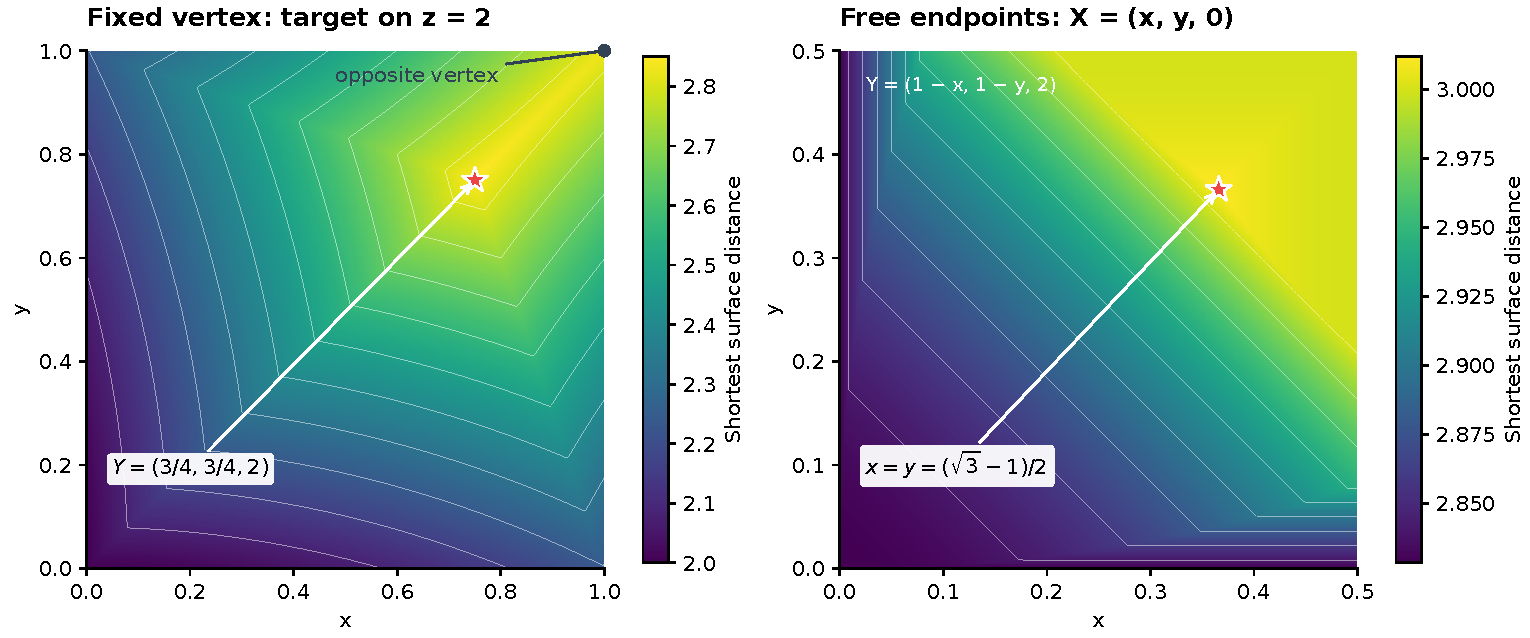
\includegraphics[width=\linewidth]{figures/distance_maps.pdf}
\caption{Exact distance formulas for the \(1\times1\times2\) box.
Left: the target moves over the face opposite a fixed vertex.
Right: the starting point moves over a quarter of the bottom face
and the target is its central reflection. The red stars are the
maximizers, not estimates from the plotted grid.}
\end{figure}

\section{Why finite unfoldings solve the continuous-path problem}
\label{sec:paths}

We first justify the geometric reductions; otherwise a list of nets can
silently miss paths or admit straight lines that do not fold to surface paths.

\subsection{Existence and finite face sequences}

There is a minimizing surface path between any two surface points.
Here is a finite-dimensional way to see this without assuming a smooth
surface. Given any continuous surface curve, a portion joining two
points of one closed face can be replaced by their straight chord in
that face. Its length does not increase.

More explicitly, start at time \(t=0\). Choose a face containing
\(\gamma(t)\) that the remaining curve visits at some later time, and
let \(t'\) be its last visit. Replace the portion from \(t\) to \(t'\)
by its chord. Unless \(t'=1\), some face containing \(\gamma(t')\)
is visited at times immediately after \(t'\): this follows by taking a
sequence of later times and using that there are only six closed faces.
Choose such a face next and repeat. A face chosen earlier cannot be
chosen again after its last-visit time. Consequently this process ends
in at most six steps. Constant terminal portions cause no problem.
It produces a polygonal surface path no longer than the original curve,
supported by a face sequence with no repetition.

There are finitely many such face sequences. For a fixed sequence,
the crossing points range over a product of closed shared edges,
which is compact; the sum of Euclidean segment lengths is continuous.
Every nonempty choice therefore has a minimum. Taking the minimum over
the finite family produces a surface path attaining the infimum over
all continuous paths. This argument also covers infinite-length input
curves, which cannot improve an already available finite path.

A shortest path cannot leave a face and subsequently return to it.
Otherwise replace that excursion by its chord. Equality in the
Euclidean chord-versus-length inequality forces the entire excursion
to be the straight chord, contradicting its departure from the face.
Thus the no-repetition reduction also describes a shortest path itself,
up to choices of the supporting face for a segment on an edge.

\subsection{Straightness, vertices, and compactness}

An ordinary edge point has a neighborhood isometric, after unfolding,
to a planar neighborhood. Hence a shortest path becomes a straight
line there, as it does in the interior of a face.

A box vertex cannot occur in the interior of a shortest path.
The total cone angle at a vertex is \(3\pi/2\). Two path rays through
it divide this angle into sectors, one of angle at most \(3\pi/4<\pi\).
Develop that sector and replace the two short radial segments by
their planar chord. The chord remains in the sector and is strictly
shorter. This contradiction excludes the vertex.

Successive development of the visited faces therefore turns a shortest
path into one straight segment. Conversely, a straight segment in a
development gives a surface path only if it crosses the actual shared
edges in the required order and stays inside the developed faces.
We check that condition below.

The intrinsic topology is the usual topology on the surface.
Within a face the metrics agree; an edge unfolds locally to a plane;
and a vertex has a finite Euclidean cone neighborhood. These charts
give local equivalence of distances. The surface is compact in this
topology, and the distance function is continuous by the triangle
inequality. Thus the fixed-point maxima and the diameter used here
are attained.

\section{Proof of the fixed-vertex answer}

\subsection{Only the face perpendicular to the longest edge needs optimization}

A point sharing a face with \(O\) has its straight Euclidean segment
to \(O\) on that face, so its distance is at most
\(\sqrt{b^2+c^2}<\sqrt{\sqzero}\).

For \((a,y,z)\), unfold the faces \(y=0\) and \(x=a\).
This gives an admissible path of length
\[
\sqrt{(a+y)^2+z^2}\le\sqrt{(a+b)^2+c^2}.
\]
For \((x,b,z)\), use \(x=0\) followed by \(y=b\); the analogous
bound is \(\sqrt{(b+x)^2+z^2}\le\sqrt{\sqzero}\).
Both bounds are strict unless the point is \(V=(a,b,c)\).
It remains to optimize over the top face
\[
T=\{(x,y,c):0\le x\le a,\ 0\le y\le b\}.
\]

\subsection{An exhaustive source-image table}

Write \(F_x,F_y,F_z\) for the faces with the respective coordinate
zero, and \(G_x,G_y\) for \(x=a,y=b\). Use planar coordinates
\((x,y)\) on \(T\). A shortest path from \(O\) that later touches a
face containing \(O\) must have stayed on that face up to that time:
compare its prefix with the straight chord from \(O\). We may therefore
represent it as starting in one source face and subsequently using only
distinct opposite faces. The complete list of possible developed
images of \(O\) is:

\begin{center}
\begin{tabular}{c l c}
\toprule
Image&Face sequence&Source coordinates in the plane of \(T\)\\
\midrule
\(A\)&\(F_x,T\)&\((-c,0)\)\\
\(B\)&\(F_y,T\)&\((0,-c)\)\\
\(C\)&\(F_y,G_x,T\)&\((a+c,-a)\)\\
\(D\)&\(F_x,G_y,T\)&\((-b,b+c)\)\\
\(E\)&\(F_z,G_x,T\)&\((2a+c,0)\)\\
\(F\)&\(F_z,G_y,T\)&\((0,2b+c)\)\\
\(P\)&\(F_y,G_x,G_y,T\)&\((2a+b,b+c)\)\\
\(Q\)&\(F_x,G_y,G_x,T\)&\((a+c,a+2b)\)\\
\(R\)&\(F_z,G_x,G_y,T\)&\((a+b,a+b+c)\)\\
\(S\)&\(F_z,G_y,G_x,T\)&\((a+b+c,a+b)\)\\
\bottomrule
\end{tabular}
\end{center}

For instance, unfolding \(G_x\) across \(x=a\) sends
\((a,y,z)\) to \((a+c-z,y)\). Unfolding \(F_y\) next sends \(O\)
to \((a+c,-a)\), the third row. All rows follow from the same
right-angle development. The possible next faces are fully enumerated
because opposite parallel faces are not adjacent. Degenerate edge
paths belong to shorter rows or their limits.

For an image \(Z\), let \(f_Z(x,y)=|(x,y)-Z|^2\). The following
identities eliminate the last six rows:
\begin{align*}
f_E-f_C&=2a[(a-x)+(b-y)+(c-b)],\\
f_F-f_D&=2b[(a-x)+(b-y)+(c-a)],\\
f_P-f_D&=4(a+b)(a-x),\\
f_Q-f_C&=4(a+b)(b-y),\\
f_R-f_D&=2[a(c-b)+(a+2b)(a-x)+a(b-y)],\\
f_S-f_C&=2[b(c-a)+b(a-x)+(2a+b)(b-y)].
\end{align*}
Every right side is nonnegative on the target rectangle. Thus any
shortest path has squared length at least the minimum of the first
four source-image distances.

\subsection{Validity of the four retained images}

The lines from \(A\) and \(B\) are always valid in their two-face nets.
For \(C\), the correct three-face crossing condition is
\[
ax+cy\ge a^2.
\]
Indeed the line from \(C=(a+c,-a)\) to \((x,y)\) crosses \(y=0\)
at horizontal coordinate
\[
\frac{(a+c)y+ax}{a+y}.
\]
It belongs to the required edge precisely when it is at least \(a\).
The subsequent crossing of \(x=a\) is then also in its edge, and
convexity of the three rectangles keeps the intervening pieces inside.

If the condition fails, then \(y<a(a-x)/c\), and
\[
f_C-f_B=2[(a+c)(a-x)-(c-a)y]>0.
\]
For example, the bracket is at least
\((a-x)(c+a^2/c)>0\) under this failure condition.
So an invalid \(C\)-line cannot be a minimum.

Similarly, \(D\) is valid precisely when \(cx+by\ge b^2\).
If this fails, \(x<b(b-y)/c\) and
\[
f_D-f_A=2[(b+c)(b-y)-(c-b)x]>0.
\]
Consequently the minimum of the four retained quantities always
corresponds to a genuine surface path. We have proved
\begin{equation}\label{eq:four}
\begin{split}
\dist(O,(x,y,c))^2=\min\{&
(x+c)^2+y^2,\quad x^2+(y+c)^2,\\
&(a+c-x)^2+(a+y)^2,\quad
(b+x)^2+(b+c-y)^2\}.
\end{split}
\end{equation}
In particular, substituting \((x,y)=(a,b)\) proves that opposite
vertices are at distance \(\sqrt{\sqzero}\).

\subsection{Maximizing the four-image minimum}

Partition the rectangle into nearest-image Voronoi cells. A cell is
defined by inequalities \(f_Z\le f_{Z'}\); their differences are
affine, so each cell is a convex polygon, possibly degenerate.
On that cell the squared distance is the strictly convex quadratic
\(f_Z\). A convex function on a polygon attains a maximum at a vertex:
express any point as a convex combination of the polygon's vertices
and use convexity. Strict convexity excludes any nontrivial
combination from being an additional maximum.

On the boundary of the rectangle, \eqref{eq:four} simplifies to
\[
\begin{array}{c|c}
x=0&c^2+y^2\\
y=0&c^2+x^2\\
x=a&c^2+(a+y)^2\\
y=b&c^2+(b+x)^2
\end{array}
\]
and its maximum there is \(\sqzero\), attained only at \((a,b)\).
For example, at \(x=a\),
\[
f_A-f_C=2a(c-y),\quad f_B-f_C=2(c-a)y,\quad
f_D-f_C=2(a+b+c)(b-y),
\]
so \(C\) is a closest image; the other edges are checked in the same way.

An interior Voronoi vertex has at least three closest images.
Two useful identities are
\[
f_A-f_B=2c(x-y),\qquad
f_D-f_C=2(a+b+c)(x-y+b-a).
\]
Solving the two possible nearest-image triples gives
\[
U=(t,t),\qquad t=\frac{a(a+c)}{2c},
\]
from \(f_A=f_B=f_C\), and
\[
W_{\rm face}=(a-\delta,b-\delta)
\]
from \(f_A=f_C=f_D\).
They belong to the rectangle, and the fourth image is no closer:
at \(U\), \(f_D-f_C=2(a+b+c)(b-a)\ge0\); at \(W_{\rm face}\),
\(f_B-f_A=2c(b-a)\ge0\).

There are no other nearest-image triples. For \(a<b\), the triple
\(A,B,D\) would have \(x=y\), where \(C\) is strictly closer than \(D\).
The triple \(B,C,D\) would have \(y-x=b-a\), where \(A\) is strictly
closer than \(B\). If \(a=b\), the two valid points coincide and all
four images tie there.

Substitution gives
\[
f(U)=\frac{(a^2+c^2)(a^2+2ac+2c^2)}{2c^2}
\le
f(W_{\rm face})=\sqone.
\]
The inequality is strict when \(a<b\). Thus the global maximum is
\(\max\{\sqzero,\sqone\}\). Factorization \eqref{eq:vertex-factor}
proves Theorem~\ref{thm:vertex}; strict convexity and the boundary
analysis give its assertion about all farthest points.

\section{Why a diametral pair must be centrally opposite}
\label{sec:antipodal}

Symmetry alone would not justify restricting both endpoints. We prove
the needed assertion. The central reflection
\[
I(p)=(a,b,c)-p
\]
is a fixed-point-free isometry of the surface. The surface is a
topological sphere: radial projection from the center gives an explicit
homeomorphism with \(S^2\).

\begin{proposition}\label{prop:all-antipodal}
Every pair of surface points realizing the intrinsic diameter of a
cuboid is of the form \(p,I(p)\).
\end{proposition}
\begin{proof}
Choose a diametral pair \(p,q\), with distance \(D\), and suppose
\(q\ne I(p)\). Let \(\alpha\) be a shortest arc from \(p\) to \(I(p)\).
Neither \(q\) nor \(I(q)\) lies on \(\alpha\) or \(I(\alpha)\):
otherwise a proper subarc would have to have length at least \(D\),
although the full arc has length at most \(D\).

Among antipodal pairs \(r,I(r)\) on \(\alpha\), choose a pair at
smallest distance, and let \(\beta\) be the subarc between them.
This minimum exists by compactness, and is positive because \(I\)
has no fixed point. The arcs \(\beta\) and \(I(\beta)\) meet only
at their endpoints. Any additional intersection would yield a proper,
shorter antipodal subarc. Their union \(J\) is therefore a simple
closed polygonal curve.

The Jordan--Schoenflies theorem on the sphere gives two complementary
open disks, with closed-disk closures. Reflection \(I\) exchanges the
two disks. If it preserved one, Brouwer's fixed-point theorem applied
to its closure would give a fixed point of \(I\), a contradiction.
It follows that \(q\) and \(I(q)\) are on different sides of \(J\).
A shortest arc \(\gamma\) from \(q\) to \(I(q)\) meets \(J\).
After reflecting an arc if necessary, take an intersection point
\(t\in\alpha\cap\gamma\).

The triangle inequality and subarc additivity yield
\[
\begin{aligned}
2D&=\dist(p,q)+\dist(Ip,Iq)\\
&\le\dist(p,t)+\dist(t,q)+\dist(Ip,t)+\dist(t,Iq)\\
&=\dist(p,Ip)+\dist(q,Iq)\le2D.
\end{aligned}
\]
All inequalities are equalities. This already proves that an
antipodal pair attains the diameter.

For the stronger statement, \(t\) is interior to both arcs. If, for
example, \(t=p\), it is an interior point of the \(q\)-to-\(I(q)\)
arc, so \(\dist(q,p)\) would be strictly smaller than its total length,
which is at most \(D\). The other endpoint possibilities are identical.
An interior point of a shortest arc cannot be a box vertex, by
Section~\ref{sec:paths}.

Equality also makes the concatenation \(p\to t\to q\) shortest.
In a flat chart at \(t\), its direction toward \(q\) must agree with
the continuation of \(\alpha\) toward \(I(p)\). Straight continuation
through faces and ordinary edges is unique, so these two portions
coincide until one ends. They have equal lengths, because both
complete paths from \(p\) have length \(D\). Thus they end at the
same point: \(q=I(p)\), the contradiction.
\end{proof}

The Jordan--Brouwer part is the standard antipodal-existence argument
for length-metric spheres with a free involutive isometry
\cite{Nikonorov2018}. The flat local continuation argument supplies the
stronger cuboid statement used in the strict comparison.

\subsection{Restriction to the two \texorpdfstring{\(a\times b\)}{a x b} faces}

Suppose an antipodal pair lies off both \(z=0\) and \(z=c\).
Its heights are \(z,c-z\) with \(0<z<c\). Parameterize the four
lateral faces by perimeter coordinate modulo \(2(a+b)\) and height.
Central reflection shifts the perimeter coordinate by \(a+b\).
The straight path in a half-belt unfolding has length
\[
\sqrt{(a+b)^2+(c-2z)^2}<\sqrt{(a+b)^2+c^2}.
\]
The right side is already attained by opposite vertices. Hence such
a pair cannot be diametral.

Reflecting in coordinate midplanes, the remaining search is exactly
\begin{equation}\label{eq:quarter}
M=(x,y,0),\quad N=(a-x,b-y,c),\qquad
0\le x\le a/2,\quad 0\le y\le b/2.
\end{equation}

\section{The five antipodal unfolding distances}
\label{sec:five}

For the points in \eqref{eq:quarter}, set
\begin{align}
d_1^2&=(a+c)^2+(b-2y)^2,&
d_2^2&=(b+c)^2+(a-2x)^2,\notag\\
d_3^2&=(c+x+y)^2+(a+b-x-y)^2,\label{eq:five}\\
d_4^2&=(a+b)^2+(c+2y)^2,&
d_5^2&=(a+b)^2+(c+2x)^2.\notag
\end{align}

\begin{lemma}\label{lem:five}
The exact antipodal distance is
\[
\dist(M,N)=\min\{d_1,d_2,d_3,d_4,d_5\}.
\]
\end{lemma}
\begin{proof}
Between the initial bottom-face and final top-face pieces, a shortest
path traverses consecutive lateral faces, without repetition.
Four lateral faces are unnecessary. In the developed lateral belt,
the horizontal displacement of a route crossing all four is at least
\(a+b\): the two complete middle faces have total width \(a+b\).
The complementary direction around the belt has displacement at most
\(a+b\), the same vertical displacement \(c\), and uses fewer faces.
Replacing just this belt portion does not increase the length.

For completeness, there are \(4,8,8,8\) simple bottom-to-top face
sequences with respectively one, two, three, or four lateral faces.
The last group has just been eliminated. Put \(A_0=a+b\) and
\(f(q)=(c+q)^2+(A_0-q)^2\). Reflection across successive shared
edges gives the following distinct squared lengths; reversing an
antipodal path duplicates an entry.

\begin{center}
\begin{tabular}{c p{11cm}}
\toprule
Lateral faces&All distinct developed squared lengths\\
\midrule
One&\(d_1^2,\ d_2^2\)\\[2pt]
Two&\(f(x+y),\ f(A_0-x-y),\ f(a-x+y),\ f(b+x-y)\)\\[2pt]
Three&\(A_0^2+(c+2y)^2,\ A_0^2+(c+2(b-y))^2,\)
\newline
\(A_0^2+(c+2x)^2,\ A_0^2+(c+2(a-x))^2\)\\
\bottomrule
\end{tabular}
\end{center}

Each alternative argument \(q\) in the two-face row is at least
\(q_0=x+y\), and
\[
f(q)-f(q_0)=2(q-q_0)(c+q+q_0-A_0).
\]
The last factor is respectively \(c\), \(c-b+2y\), or \(c-a+2x\),
all nonnegative. Thus \(d_3^2=f(x+y)\) dominates that row.
In the three-face row, \(x\le a/2\) and \(y\le b/2\) eliminate the
two larger alternatives. This gives a lower bound by the minimum
of the five retained expressions.

We must still exclude artificially short, invalid straight lines.
The \(d_1,d_2\) routes, using one lateral face, are always valid.
The following checks cover all other possibilities.

\emph{The \(d_3\) route.}
Develop the lateral faces \(y=0\) then \(x=a\) into
\([0,a+b]\times[0,c]\). The endpoints develop to
\((x,-y)\) and \((a+b-y,c+x)\). Edge-crossing conditions are
\[
x(a-x)\le(b-y)(c+y),\qquad
y(b-y)\le(a-x)(c+x).
\]
The first always holds: its left side is at most \(a^2/4\) and
its right side is at least \(3b^2/4\).
If the second fails, put
\(\Delta=y(b-y)-(a-x)(c+x)>0\). Expansion gives
\[
d_3^2-d_1^2=
2\Delta+2\{y(c-a+2x)+b(a-x)\}>0.
\]
An invalid \(d_3\) is therefore longer than the valid \(d_1\).

\emph{The \(d_4\) route.}
Use successive lateral strip widths \(a,b,a\); the developed
endpoints are \((x,-y)\) and \((a+b+x,c+y)\).
Let \(r=(a+b)y/(c+2y)\). Validity is exactly
\(r\le x\le a-r\). On our quarter-face, failure implies \(x<r\).
For fixed \(y\), the difference \(d_4^2-d_3^2\) is a concave
quadratic in \(x\), with second derivative \(-4\). Its values at
the two endpoints of \([0,r]\) are
\[
2y(a+b+c+y)
\quad\text{and}\quad
\frac{2y(c+y)\{(a+b)^2+(c+2y)^2\}}{(c+2y)^2}.
\]
They are positive if \(y>0\), so the difference is positive
throughout that interval. If \(y=0\), then \(r=0\) and no failure
is possible. An invalid \(d_4\) is thus longer than \(d_3\);
if \(d_3\) is itself invalid, it is in turn longer than \(d_1\).

\emph{The \(d_5\) route.}
Exchange \((a,x)\) with \((b,y)\) in the preceding argument.
Its validity failure likewise makes it longer than \(d_3\).

Consequently an expression attaining the five-term minimum always
has a valid surface realization. This proves the reverse bound and
the equality.
\end{proof}

\section{Solving the unrestricted optimization}
\label{sec:rootproof}

\subsection{A one-dimensional necessary bound}

Take a target squared length \(T>\sqzero\), and write
\[
u_T=\spq{T-(b+c)^2},\quad
v_T=\spq{T-(a+c)^2},\quad
t_T=\sqrt{2T-(a+b+c)^2}.
\]
If all five squared lengths in \eqref{eq:five} are at least \(T\),
the first two imply
\[
x\le\frac{a-u_T}{2},\qquad y\le\frac{b-v_T}{2}.
\]
The third can be written
\[
d_3^2=\frac{(a+b+c)^2+(c-a-b+2x+2y)^2}{2}.
\]
Since \(T>\sqzero\), we have \(t_T>|a+b-c|\).
The negative square-root branch would force \(x+y<0\), so
\[
x+y\ge\frac{a+b-c+t_T}{2}.
\]
Combining the bounds yields the necessary condition
\[
u_T+v_T+t_T\le c,\qquad\text{or equivalently}\qquad F(T)\le c.
\]

The function \(F\) is continuous and strictly increasing because its
first two terms are nondecreasing and its last term is strictly
increasing. At
\[
U_0=(a+c)^2+b^2
\]
we have
\[
\sqrt{2U_0-(a+b+c)^2}=a+c-b,\qquad
F(U_0)=a+c+\spq{U_0-(b+c)^2}>c.
\]
Thus if \(F(\sqzero)\ge c\), nothing exceeds \(\sqrt{\sqzero}\).
If \(F(\sqzero)<c\), there is a unique
\(T_*\in(\sqzero,U_0)\) with \(F(T_*)=c\), and nothing exceeds
\(\sqrt{T_*}\).

\subsection{The root supplies a maximizing pair}

Use \(u,v,x,y\) from \eqref{eq:witness}, and put
\[
t=\sqrt{2T_*-(a+b+c)^2}.
\]
Then \(u+v+t=c\).
Because \(T_*<U_0\le(b+c)^2+a^2\), we have \(u<a\) and \(v<b\).
It follows that \(x>0,y>0\), with \(x\le a/2,y\le b/2\).
The first two squared route lengths are at least \(T_*\),
and the equation \(u+v+t=c\) gives \(d_3^2=T_*\).
It remains to check \(d_4,d_5\); ignoring them would leave a gap.

First \(T_*>(a+c)^2\), so \(v>0\) and
\(T_*=(a+c)^2+v^2\). This is immediate if \((a+c)^2<\sqzero\).
Otherwise, at \(T=(a+c)^2\) the first two radicals of \(F\)
vanish, and
\[
[2T-(a+b+c)^2]-c^2
=a^2-b^2+2c(a-b)-2ab<0.
\]
Hence \(F(T)<c\) there, and the root is larger.

Define
\[
v_0=b-\frac{a(c-b)}{b+c}>0,\qquad
h(z)=z^2+2cz+a^2-b^2+2c(a-b)-2ab.
\]
Since \(t=c-u-v\),
\[
h(v)=t^2-(c-v)^2\le0.
\]
The polynomial \(h\) is strictly increasing for nonnegative inputs,
whereas exact substitution gives
\[
h(v_0)=\frac{2a^2(b^2+c^2)}{(b+c)^2}>0.
\]
Thus \(v<v_0\), and
\begin{equation}\label{eq:slack4}
d_4^2-T_*
=2\{(b+c)(b-v)-a(c-b)\}>0.
\end{equation}

If \(u=0\), then
\[
d_5^2-T_*=(a+b)^2-v^2>0
\]
because \(v<b\).
If \(u>0\), use \(T_*=(b+c)^2+u^2\) and set
\[
k(z)=z^2+2cz+b^2-a^2+2c(b-a)-2ab,\qquad
w=a-\frac{b(c-a)}{a+c}.
\]
Now
\[
k(u)=t^2-(c-u)^2<0,
\]
since \(v>0\). Consequently \(k(0)<0\). The identity
\[
k(0)=a^2+b^2-2(a+c)w
\]
shows that \(w>0\). Finally,
\[
k(w)=\frac{2b^2(a^2+c^2)}{(a+c)^2}>0.
\]
Monotonicity gives \(u<w\), so
\begin{equation}\label{eq:slack5}
d_5^2-T_*
=2\{(a+c)(a-u)-b(c-a)\}>0.
\end{equation}
The five-route minimum is therefore exactly \(\sqrt{T_*}\).
This proves Theorem~\ref{thm:diam}, including admissible coordinates.

\subsection{The strict comparison with a fixed vertex}

Always
\[
\sqrt{\sqzero}\le\vertexecc\le\diameter.
\]
If \(\diameter=\sqrt{\sqzero}\), both inequalities are equalities.
If \(\diameter>\sqrt{\sqzero}\) but \(\vertexecc=\diameter\),
a farthest point \(Y\) from \(O\) would make \((O,Y)\) a diametral
pair. Proposition~\ref{prop:all-antipodal} forces \(Y=I(O)=V\),
whose distance is only \(\sqrt{\sqzero}\), a contradiction.
Thus strict improvement occurs exactly when \(F(\sqzero)<c\).

At \(T=\sqzero\), the first two radicands in \eqref{eq:F} are
\[
b^2+2ab-2ac,\qquad a^2+2ab-2bc,
\]
and the last radical is \(|a+b-c|\).
If \(c\le a+b\), the condition \(F(\sqzero)<c\) is exactly
\eqref{eq:strict-criterion}. If \(c>a+b\), each of the first
two radicals is respectively smaller than \(b\) or \(a\), and
both criteria hold automatically. This proves
Corollary~\ref{cor:strict} in all cases.

\section{Elementary branches and a useful one-parameter family}
\label{sec:radicals}

\subsection{An explicit radical branch}

The clipped-radical equation \eqref{eq:F} is often the simplest way
to use the answer. For comparison with the traditional piecewise
formula, suppose \(F(\sqzero)<c\), and put
\[
K=(b-a)(a+b+2c).
\]
If
\[
a^2b^2\le c^2K,
\]
the root has \(u=0\). Define
\[
R=\sqrt{(b+c)^2-2a(c-b)-a^2}
  =\sqrt{c^2+K+2ab}.
\]
Then
\[
\boxed{\ x=\frac a2,\quad y=\frac{b+c-R}{2},\quad
\diameter^2=b^2+3c^2+2b(a+c)-2cR.\ }
\]
To derive this, \(u=0\) reduces the root equation to \(v+t=c\).
Squaring and using \(T=(a+c)^2+v^2\) gives
\[
v^2+2cv-K-2ab=0,
\]
whose positive solution is \(v=R-c\).
The consistency condition \(T\le(b+c)^2\) is \(v\le\sqrt K\).
Since the polynomial on the left is increasing for \(v\ge0\),
this is equivalent to \(2c\sqrt K-2ab\ge0\), as claimed.
Also \(0<v<c\): positivity is immediate, while
\(K+2ab<3c^2\) follows from \(0<a\le b\le c\).
Thus squaring has not introduced the wrong sign of \(t\).
The candidate \(T=(a+c)^2+v^2\) satisfies
\(2T-(a+b+c)^2=(c-v)^2\) and \(F(T)=c\).
The same formula defines a strictly increasing \(F\) on
\(T\ge(a+b+c)^2/2\). Since \(F(\sqzero)<c\), the candidate
must have \(T>\sqzero\), so it is the unique root already established.
If this branch condition fails, the actual root has \(u>0\).

In that remaining branch, both leading radicals are positive and
the length is the unique solution above
\(\max\{b+c,\sqrt{\sqzero}\}\) of
\[
\sqrt{D^2-(a+c)^2}+\sqrt{D^2-(b+c)^2}
 +\sqrt{2D^2-(a+b+c)^2}=c.
\]
At the boundary between the two branches, the formulas agree.
These cases agree with the published cuboid diameter
formula \cite{NN2008}.

\subsection{Square cross sections}

Let \(a=b=s\) and \(c\ge s\). The free-endpoint answer simplifies to
\[
\diameter=
\begin{cases}
\sqrt{c^2+4s^2},&s\le c\le\sqrt2\,s,\\[2pt]
\sqrt{3c^2+2sc-2c\sqrt{c^2-s^2}},&c>\sqrt2\,s.
\end{cases}
\]
In the second case choose
\[
x=y=\frac{s-c+\sqrt{c^2-s^2}}2,\quad
X=(x,x,0),\quad Y=(s-x,s-x,c).
\]
For a fixed vertex, the opposite vertex remains farthest until
\[
c=\frac{3+\sqrt{17}}4\,s\approx1.7807764064\,s.
\]
Strict improvement in the unrestricted problem begins for
\(c>\sqrt2\,s\approx1.4142135624\,s\); equality still holds at
the threshold itself.
This explains why the two questions have distinct transition tests.

\begin{figure}[htbp]
\centering
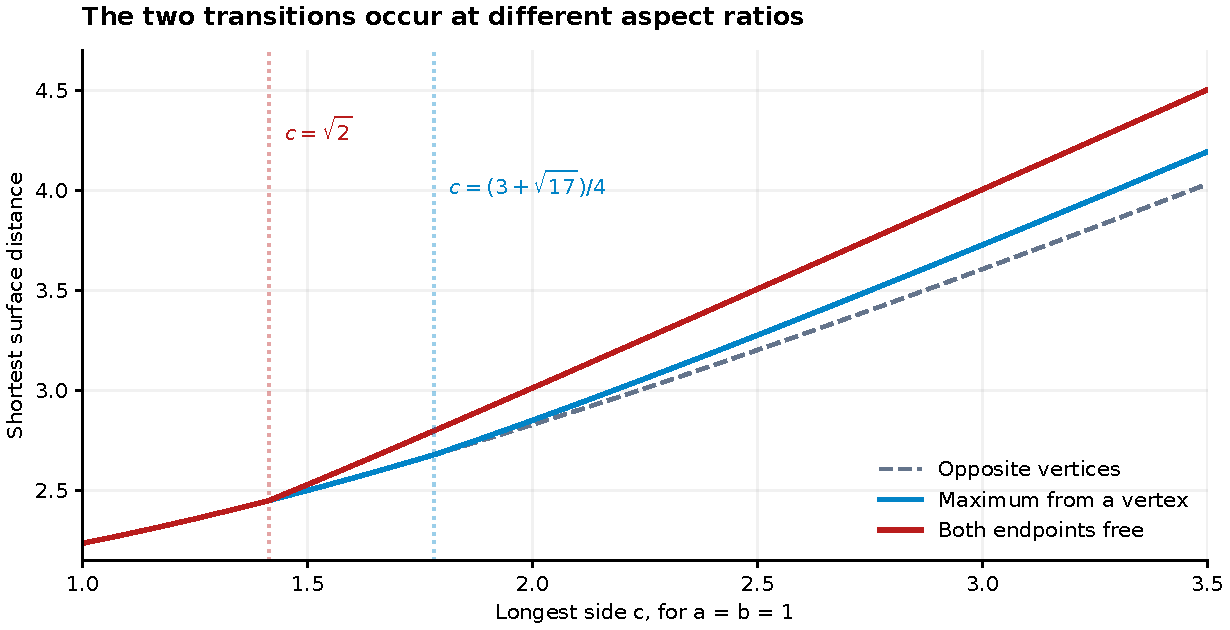
\includegraphics[width=.94\linewidth]{figures/square_family.pdf}
\caption{The family \(1\times1\times c\). The first transition concerns
the unrestricted diameter; the later one concerns the farthest point
from a vertex. All three plotted curves are exact formulas.}
\end{figure}

\section{Lean formalization: definitions, statements, and completion plan}
\label{sec:lean}

\subsection{Scope and status}

The accompanying \texttt{lean/CuboidSurface.lean} is a formalization
outline, not a completed proof. It has explicit definitions and named
remaining proof obligations. It is marked uncompiled because the
execution environment did not contain Lean or Lake. No assertion of
kernel-checked correctness is made for that file.

The current task does not impose an iPRA restriction. The appropriate
target is ordinary Lean 4 real Euclidean geometry with mathlib. A
narrow read-only inspection of ProveIt found no directly reusable
completed cuboid surface-distance theorem. Its Cauchy--residue iPRA
report discusses controlled rectifiable curves, but marks the associated
Lean material as an uncompiled candidate \cite{ProveIt}. Consequently
the proposed development uses explicit definitions and verified
mathlib interfaces, rather than treating an outline as an established
dependency.

The checked API reference is mathlib commit
\texttt{6c9a0a07bbbce9b0205b16c83a17b8458f4bcdf9},
whose toolchain is Lean \texttt{v4.36.0}.
The files \texttt{PiL2.lean}, \texttt{BoundedVariation.lean},
and \texttt{ConstantSpeed.lean} provide the relevant Euclidean-space,
variation, and constant-speed interfaces \cite{Mathlib}.

\subsection{Foundational definitions}

Use \(\mathrm{E3}=\texttt{EuclideanSpace}\ \R\ (\texttt{Fin}\ 3)\).
The Euclidean norm matters: a plain function space can carry a
supremum norm instead. Coordinate vectors in the pinned API can be
written using its \(L^2\) vector notation.

For a length vector \(L\), define
\[
\begin{split}
\operatorname{OnSurface}(L,p)\ \Longleftrightarrow\
&(\forall i,\ 0\le p_i\le L_i)\\
&{}\land(\exists i,\ p_i=0\ \lor\ p_i=L_i).
\end{split}
\]
An admissible curve is a function
\(\gamma:\R\to\mathrm{E3}\) continuous on \([0,1]\), with the
specified endpoints and all values on that interval on the surface.
Its extended length is
\[
\texttt{eVariationOn}\ \gamma\ (\texttt{Set.Icc}\ 0\ 1)
\quad\text{in }\R_{\ge0}\cup\{\infty\}.
\]
Define the extended intrinsic distance as the infimum of the set of
these lengths. Prove it is finite using explicit polygonal surface
paths before converting it to a real number with
\texttt{ENNReal.toReal}. This order prevents an infinite distance
from being silently converted to zero.

Define a face as a coordinate index and a choice of lower or upper
endpoint. A face word is a list of faces, adjacent successively,
without repetition. A polygonal path record contains its face word,
its crossing points, endpoint equalities, and proofs that each segment
is in the appropriate closed rectangular face. The length is the
finite sum of Euclidean segment lengths.

The scalar layer contains the positive ordered side data,
\(\sqzero,\sqone,H,\delta\), the four vertex squared lengths,
the five antipodal squared lengths, and \(F\). The nonvertex
diameter is specified by its unique root in
\((\sqzero,(a+c)^2+b^2)\); the scaffold exposes the root condition
and its monotonic characterization, rather than treating a numerical
solver as an oracle.

\subsection{Proof milestones}

\begin{longtable}{p{.23\linewidth} p{.69\linewidth}}
\toprule
Milestone&Mathematical content and formal route\\
\midrule
\endhead
Curve length&
Partition sums, concatenation additivity, reversal, and invariance under
Euclidean isometries. Use \texttt{eVariationOn}; its
\texttt{Icc\_add\_Icc} lemma and finite partition bounds are relevant.
\\[4pt]
Polygonal equivalence&
Implement the last-visit argument of Section~\ref{sec:paths} for the
finite closed-face cover. It yields a face-word polygon no longer
than any admissible curve. Compact products of crossing edges give
a minimizing polygon.
\\[4pt]
Local geometry&
Closed-face convexity gives no revisits. Two-face isometries give
straightness and unique continuation at nonvertices. A
\(3\pi/2\)-cone shortening lemma excludes interior vertices.
\\[4pt]
Vertex net certificate&
Enumerate the ten rows above as a finite datatype/list. Prove the six
domination identities by ring normalization and inequalities.
Check \(C,D\) validity, then prove \eqref{eq:four}.
\\[4pt]
Vertex optimization&
Use either finite Voronoi polygons or an equivalent partition by the
affine bisectors. Enumerate their vertices, bound convex quadratics
by vertex values, and normalize the two circumcenter formulas.
Finish with \eqref{eq:vertex-factor}.
\\[4pt]
Antipodal diameter&
Formalize the invariant Jordan curve and disk-exchange argument,
then equality in the triangle inequality and flat continuation.
This is the main topological obligation, not an algebra tactic.
The radial sphere homeomorphism is explicit.
\\[4pt]
Antipodal net certificate&
Enumerate the 28 simple bottom-to-top words, remove four-lateral-face
routes by the belt replacement, and verify the ten distance families,
the dominance tests, and the invalid-route inequalities.
\\[4pt]
Scalar optimization&
Use nonnegative square-root identities and monotonicity to derive
\(F(T)\le c\). Apply the intermediate value theorem and strict
monotonicity for the unique root. The two slack calculations
\eqref{eq:slack4}--\eqref{eq:slack5} give attainment.
\\[4pt]
Final comparison&
Compactness supplies a farthest point. Combine the diameter theorem
with the assertion that all diametral pairs are antipodal to obtain
the strict-improvement equivalence.
\\
\bottomrule
\end{longtable}

No numerical validation replaces a milestone in this table.
The scalar algebra is suited to \texttt{ring}, \texttt{field\_simp},
\texttt{linarith}, and \texttt{nlinarith}, after explicitly recording
positive denominators and square-root sign conditions.
The finite geometry should be certified as a complete enumeration,
including invalid paths, not assumed from a diagram.

If the required topological library lemmas are unavailable in the
chosen mathlib revision, a separate development of polygonal Jordan
separation and Brouwer for a closed disk is needed. An alternative,
larger project is a cuboid-specific finite certificate bounding all
pairs of endpoint faces directly; that would bypass the general
antipodal theorem. The present scaffold follows the geometric proof
above and leaves this obligation visible.

\section{Reproducible artifacts and verification}
\label{sec:artifacts}

The archive is self-contained apart from standard software dependencies:

\begin{itemize}
\item \texttt{cuboid\_surface.tex} and \texttt{cuboid\_surface.pdf}:
the complete report and its compiled version.
\item \texttt{code/cuboid.py}: standard-library, high-precision
decimal evaluation of both answers, with coordinates restored to the
input axis order. It uses monotone bisection, not a surface grid.
\item \texttt{code/unfold\_verify.py}: an independent, standard-library
enumeration of every simple face chain. It unfolds the faces, checks
the actual edge intersections and face containment, and returns a
shortest valid path with three-dimensional crossing coordinates.
\item \texttt{code/validate.py}: reproducible comparison of the two
independent algorithms and known-answer tests.
\item \texttt{code/verify\_algebra.py}: exact SymPy checks of
18 displayed rational or polynomial identities.
\item \texttt{code/make\_figures.py} and \texttt{figures/}: reproducible
scientific figures in vector PDF and PNG form.
\item \texttt{lean/}: the explicitly unfinished Lean outline,
toolchain information, and completion notes.
\item \texttt{verification/}: executed numerical and symbolic results.
\end{itemize}

The independent checks covered 18 boxes, including asymmetric,
elongated, thin, transition-near, and permuted-axis examples.
There were 216 comparisons of maximizing witnesses and arbitrary
top-face or antipodal points, plus 10 known-answer cases.
All passed. The largest absolute distance discrepancy was
\(7.11\times10^{-15}\); the largest discrepancy divided by the
maximum of \(1\) and the expected distance was
\(4.12\times10^{-16}\).
The lifted path segment sums also matched the developed lengths.
All 18 symbolic identities simplified exactly to zero.

The independent unfolding program uses floating-point tolerances;
its results are numerical checks, not interval certificates.
In particular, distinctions at its tolerance scale or extremely thin
boxes require higher precision. The proof establishes the exact results
for all positive side lengths. The Decimal root bracket in the
calculator is likewise a high-precision numerical result, with no
claim of directed-rounding certification.

Example commands, run from the extracted directory:
\begin{lstlisting}
python3 code/cuboid.py 1 1 2
python3 code/unfold_verify.py --sides 1 1 2 \
  --p 0 0 0 --q .75 .75 2
python3 code/validate.py
python3 code/verify_algebra.py
python3 code/make_figures.py
latexmk -pdf -interaction=nonstopmode cuboid_surface.tex
\end{lstlisting}

\begingroup
\small\raggedright
\begin{thebibliography}{9}

\bibitem{NN2008}
Y.~G. Nikonorov and Y.~V. Nikonorova,
\emph{The Intrinsic Diameter of the Surface of a Parallelepiped},
Discrete \& Computational Geometry \textbf{40} (2008), 504--527.
\href{https://doi.org/10.1007/s00454-007-9037-7}
{doi:10.1007/s00454-007-9037-7}.
Full text:
\url{https://link.springer.com/content/pdf/10.1007/s00454-007-9037-7.pdf}.

\bibitem{Nikonorov2018}
Yu.~G. Nikonorov,
\emph{On the geodesic diameter of surfaces with involutive isometry},
arXiv:1811.01173 (2018), English translation of the 2001 paper in
Trudy Rubtsovsk Industrial Institute \textbf{9}, 62--65.
\url{https://arxiv.org/abs/1811.01173}.
Author-uploaded text was also checked on ResearchGate.

\bibitem{MillerSchaefer}
S.~Michael Miller and Edward F. Schaefer,
\emph{The distance from a point to its opposite along the surface of a box},
Pi Mu Epsilon Journal \textbf{14} (2015), 143--154.
\url{https://arxiv.org/abs/1502.01036}.
This is additional background on antipodal unfoldings.

\bibitem{ProveIt}
Vladimir Reshetnikov, \emph{ProveIt}, GitHub repository.
\url{https://github.com/VladimirReshetnikov/ProveIt}.
Read-only review on 19 November 2026, including
\texttt{Logic/PrimitiveRecursiveArithmetic/docs/proofs/analysis/}
\texttt{cauchy\_residue\_ipra/README.md}.
The narrow search is not a claim that no related material exists elsewhere.

\bibitem{Mathlib}
The mathlib community, \emph{mathlib4}, revision
\texttt{6c9a0a07bbbce9b0205b16c83a17b8458f4bcdf9}.
\url{https://github.com/leanprover-community/mathlib4}.
Verified interfaces:
\texttt{Mathlib/Analysis/InnerProductSpace/PiL2.lean},
\texttt{Mathlib/Topology/EMetricSpace/BoundedVariation.lean},
and \texttt{Mathlib/Analysis/ConstantSpeed.lean}.

\end{thebibliography}
\endgroup
\end{document}
